%!TEX root = tesis.tex
\chapter{Un \ssolver paralelo y distribuido }
\label{ssolver-pardist}

\begin{itemize}
	\item Escalable
	\item Uso de SAT Solver off-the-shelf
	\item Multiplataforma
	\item Tablero de control
\end{itemize}

\section{Arquitectura}
\missingfigure{Diagrama de arquitectura del solver}

\subsection{Lo del \cluster}

\subsection{El tablero de control}

\begin{figure}
	\begin{subfigure}[b]{0.5\textwidth}
		\centering
		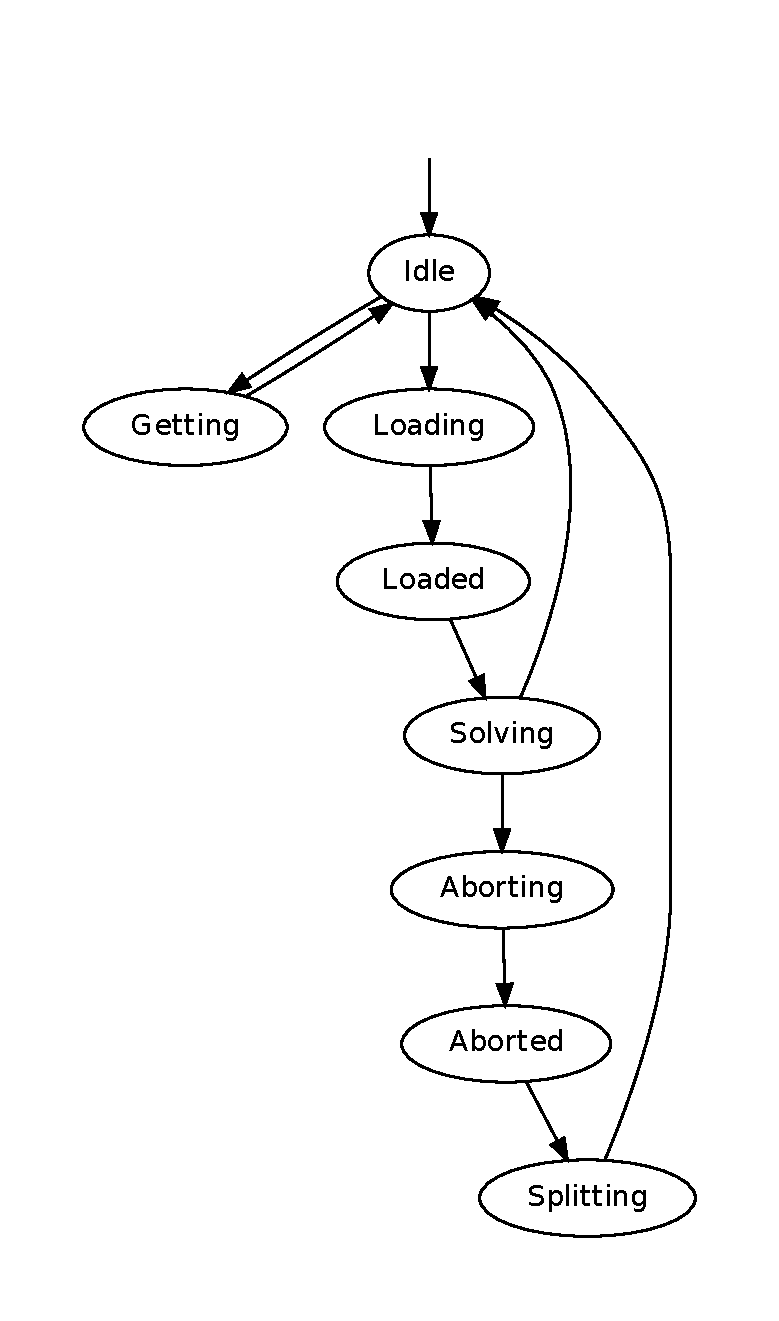
\includegraphics[scale=0.5]{graphs/workerstates}
		\caption{\emph{Workers}}
	\end{subfigure}
	\begin{subfigure}[b]{0.5\textwidth}
		\centering
		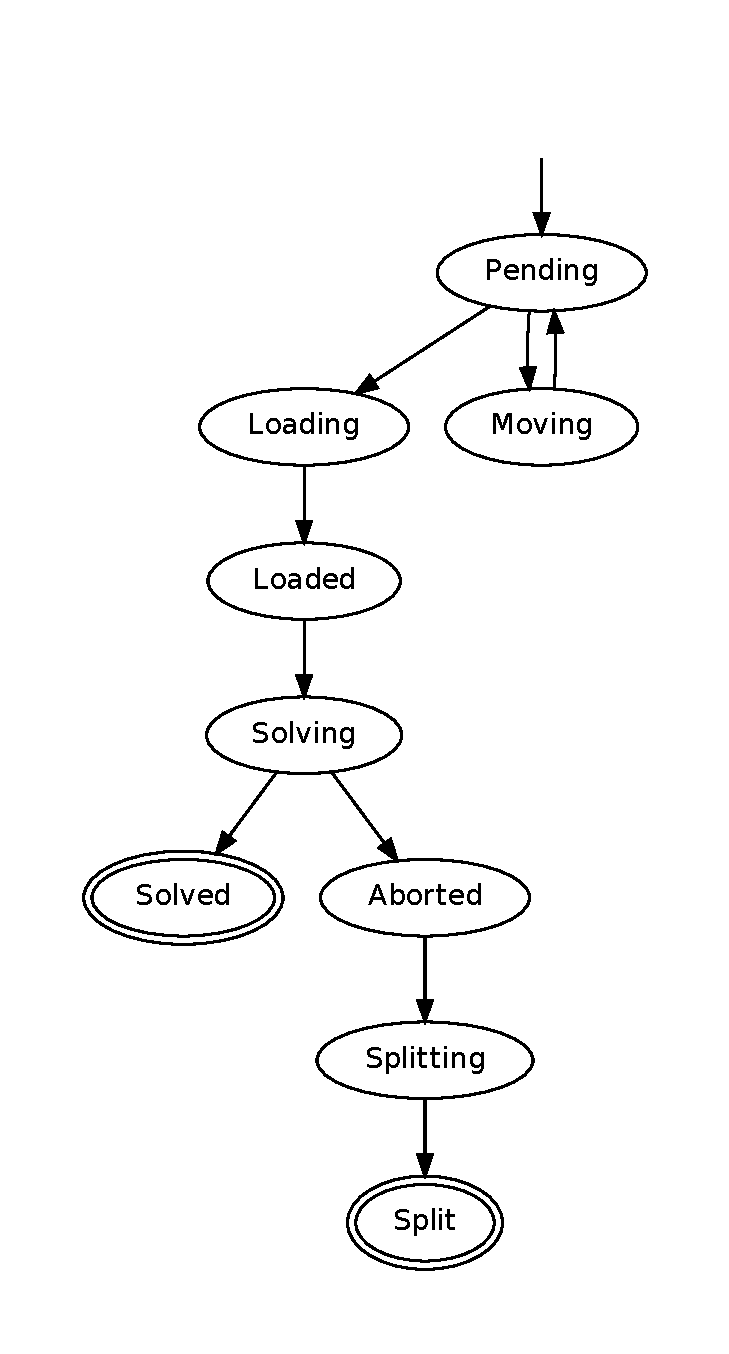
\includegraphics[scale=0.5]{graphs/taskstates}
		\caption{Tareas}
	\end{subfigure}
	\caption{Diagramas de estado en el tablero de control}
\end{figure}

\begin{small}
\begin{lstlisting}[language=Python,caption=Interfaz Strategy]
class Strategy(object):
	def register_globalstate(self, globalstate)
	def register_socket(self, commandsocket)
	def on_init(self, worker)
	def on_createroot(self, worker, task)
	def on_init_finished(self, nworkers)
	def on_getfile(self, worker, task)
	def on_file(self, worker, task)
	def on_load(self, worker, task)
	def on_unsat(self, worker, task)
	def on_sat(self, worker, task, modelstr)
	def on_abort(self, worker, task)
	def on_split_newtask(self, worker, newtask)
	def on_split_finished(self, worker, parenttask, nchildren)
	def on_shutdown(self)
\end{lstlisting}
\end{small}

\subsubsection{Nuestra estrategia}

\subsection{Decisiones que vale la pena seguir investigando}

\section{Resultados experimentales}